\chapter{Detailed Report}\label{chapter:detailed_report}

\section{Tools description}

\newpage
\section{Configuration and Deploy Management Testing}

%CONFIG 003
\simpleVulntitle{OTG-CONFIG-003}{Test File Extensions Handling for Sensitive Information}
\vultable{\doge}{%
	The batch transaction functionality at \url{http:/IPADDRESS/tran.php} does not seem to check the extension of the uploaded files.\newline
	Also, while exploring the folder structure of the server, some leftover files were found, as well as hidden folders.
}{%
	If the user tries to upload any file other than a txt file, the server does not provide any error messages. This particular vulnerability will be discussed later in 3.X.X.\newline
	Additionally, leftover files (e.g. \url{http:/IPADDRESS/employee_registration.php~}) were not deleted from the server, as well as other files containing sensitive information. More specifically, this is the case of the .git folder.
}{%
	In order to access the hidden .git folder, however, an attacker must be skilled and know where to search for sensitive information.
}{%
	Having access to the data contained inside the hidden .git folder allows to potentially get access to the whole source code of the web application.
}{%
	\cvssBaseScorePretty{N}{L}{N}{N}{C}{L}{L}{L} %FIXME: This are mock values
}
\vultable{\gnb}{%
	?
}{%
	?
}{%
	?
}{%
	?
}{%
	\cvssBaseScorePretty{N}{L}{N}{N}{C}{L}{L}{L} %FIXME: This are mock values
}
%CONFIG 006
\vulntitle{OTG-CONFIG-006}{Test HTTP Methods}
\vultable{\doge}{%
	observation text
}{%
discovery text
}{%
likelihood text
}{%
implication text
}{%
\cvssBaseScorePretty{N}{L}{N}{N}{C}{L}{L}{L} %FIXME: This are mock values
}
\vultable{\gnb}{%
	observation text
}{%
discovery text
}{%
likelihood text
}{%
implication text
}{%
\cvssBaseScorePretty{N}{L}{N}{N}{C}{L}{L}{L} %FIXME: This are mock values
}

%CONFIG 007
\vulntitle{OTG-CONFIG-007}{Test HTTP Strict Transport Security}
\vultable{\doge}{%
	The application is only accessible over HTTP.
}{%
	No HTTPS is enforced, therefore all data sent between the server and client is not encrypted.
}{%
	An attacker could perform a man in the middle attack.
}{%
	Sniffing the network traffic, all data exchanged between the server and the client can be read as clear text. No confidentiality at all is supported on this end.
}{%
	\cvssBaseScorePretty{N}{L}{N}{N}{U}{L}{L}{L} %FIXME: This are mock values
}
\vultable{\gnb}{%
	The application is only accessible over HTTP.
}{%
	No HTTPS is enforced, therefore all data sent between the server and client is not encrypted.
}{%
	An attacker could perform a man in the middle attack.
}{%
	Sniffing the network traffic, all data exchanged between the server and the client can be read as clear text. No confidentiality at all is supported on this end.
}{%
	\cvssBaseScorePretty{N}{L}{N}{N}{U}{L}{L}{L} %FIXME: This are mock values
}

%CONFIG 008
\vulntitle{OTG-CONFIG-008}{Test RIA cross domain policy}
\vultable{\doge}{%
	The web application doesn't support additional technologies like Flash, Silverlight or Java.
}{%
	No cross-domain policy files were found.
}{%
	\na
}{%
	\na
}{%
	\na
}
\vultable{\gnb}{%
	The web application doesn't support additional technologies like Flash, Silverlight or Java.
}{%
	No cross-domain policy files were found.
}{%
	\na
}{%
	\na
}{%
	\na
}

\newpage
\section{Identity Management Testing}
\simpleVulntitle{OTG-IDENT-001}{Test Role Definitions}
\vultable{\doge}{%
	Clients and non-logged in users are able to access Employee privileges, see \ref{figure:RoleDefinitionsDoge}
}{%
	This was discovered through the bug searching stage and while completing the "OTG-AUTHN-004 Testing for bypassing authentication schema" test.
}{%
	This is a relatively easy bug to uncover, so the likelihood of is quite high 
}{%
	This could have tremendous damages to the bank, as adding employee accounts and transferring functions 
}{%
\cvssBaseScorePretty{N}{L}{N}{N}{U}{L}{L}{L} %FIXME: This are mock values
}

\begin{figure}[h!tbp]
	\centering
	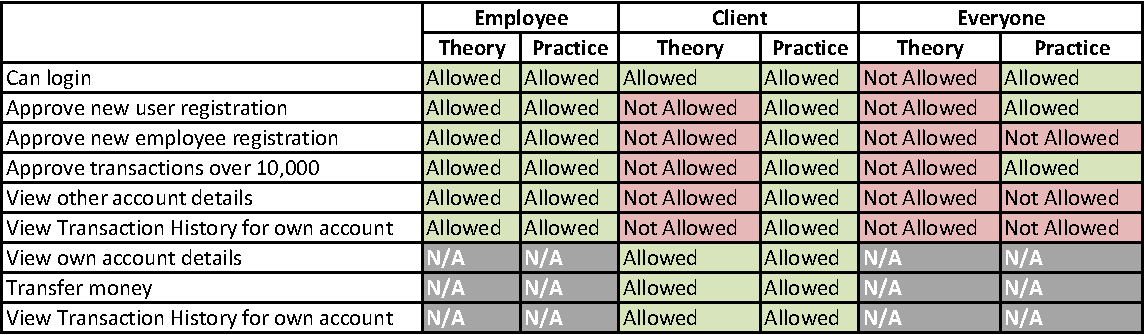
\includegraphics[width=\textwidth]{figures/RoleDefinitionsDoge}
	\caption{Role Definitions}
	\label{figure:RoleDefinitionsDoge}
\end{figure}


\vultable{\gnb}{%
	Clients, Employees and non-logged in users all act as expected, see \ref{figure:RoleDefinitionsGNB}
}{%
	This was verified through basic function testing and security testing tools (ZAP).
}{%
	N/A since no vulnerability was found.
}{%
	N/A 
}{%
\cvssBaseScorePretty{N}{L}{N}{N}{U}{L}{L}{L} %FIXME: This are mock values
}

\begin{figure}[h!tbp]
	\centering
	%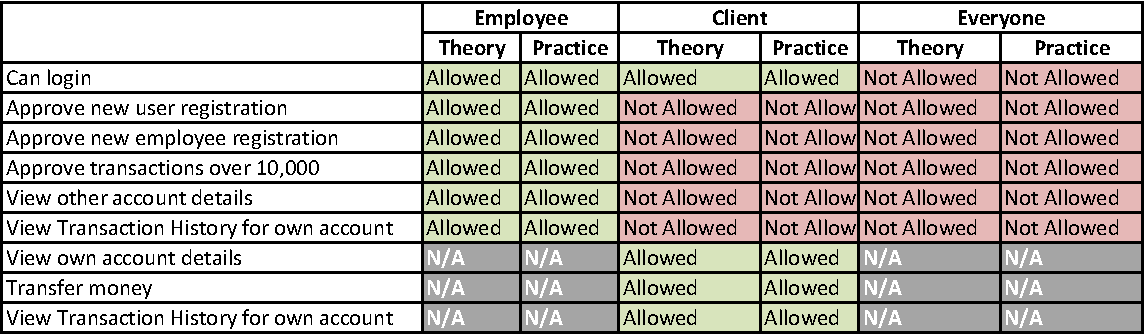
\includegraphics[width=\textwidth]{figures/RoleDefinitionsGNB}
	\caption{Role Definitions}
	\label{figure:RoleDefinitionsGNB}
\end{figure}


\vulntitle{OTG-IDENT-002}{Test User Registration Process}
\vultable{\doge}{%
	The registration process is set up for anyone to register, the process then awaits human interaction for the approval stage, this will serve an extra step of verification.

	Identities are not verified nor checked at this stage due to application limitations, email format verification is missing from the form.
}{%
	The email verification test was discovered through trail and error while registering.
}{%
	likely, due to intentional or unintentional mistyping.
}{%
	No serious impact as TAN codes are not sent to the email. 
}{%
\cvssBaseScorePretty{N}{L}{N}{N}{U}{L}{L}{L} %FIXME: This are mock values
}

\vultable{\gnb}{%
	The registration process is set up for anyone to register, the process then awaits human interaction for the approval stage, this will serve an extra step of verification.
	
	Identities are not verified nor checked at this stage due to application limitations.
}{%
	Trail and error.
}{%
	N/A since no vulnerability was found.
}{%
	N/A since no vulnerability was found. 
}{%
\cvssBaseScorePretty{N}{L}{N}{N}{U}{L}{L}{L} %FIXME: This are mock values
}

\vulntitle{OTG-IDENT-003}{Test Account Provisioning Process}
\vultable{\doge}{%
	The registration process is set up for anyone to register, the process then awaits human interaction for the approval stage, this will serve an extra step of verification.
	
	Identities are not verified nor checked at this stage due to application limitations, email format verification is missing from the form.
}{%
The email verification test was discovered through trail and error while registering.
}{%
likely, due to intentional or unintentional mistyping.
}{%
No serious impact as TAN codes are not sent to the email. 
}{%
\cvssBaseScorePretty{N}{L}{N}{N}{U}{L}{L}{L} %FIXME: This are mock values
}

\vultable{\gnb}{%
	The registration process is set up for anyone to register, the process then awaits human interaction for the approval stage, this will serve an extra step of verification.
	
	Identities are not verified nor checked at this stage due to application limitations, email format verification is missing from the form.
}{%
The email verification test was discovered through trail and error while registering.
}{%
likely, due to intentional or unintentional mistyping.
}{%
No serious impact as TAN codes are not sent to the email. 
}{%
\cvssBaseScorePretty{N}{L}{N}{N}{U}{L}{L}{L} %FIXME: This are mock values
}

\vulntitle{OTG-IDENT-004}{Testing for Account Enumeration and Guessable User Account}
\vulntitle{OTG-IDENT-005}{Testing for Weak or unenforced username policy}

\newpage
\section{Authentication Testing}	
\simpleVulntitle{OTG-AUTHN-001}{Testing for Credentials Transported over an Encrypted Channel}
\vulntitle{OTG-AUTHN-002}{Testing for default credentials}
\vulntitle{OTG-AUTHN-003}{Testing for Weak lock out mechanism}
\vulntitle{OTG-AUTHN-004}{Testing for bypassing authentication schema}
\vulntitle{OTG-AUTHN-005}{Test remember password functionality}
\vulntitle{OTG-AUTHN-006}{Testing for Browser cache weakness}
\vulntitle{OTG-AUTHN-007}{Testing for Weak password policy}
\vulntitle{OTG-AUTHN-008}{Testing for Weak security question/answer}
\vulntitle{OTG-AUTHN-009}{Testing for weak password change or reset functionalities}
\vulntitle{OTG-AUTHN-010}{Testing for Weaker authentication in alternative channel}

\newpage
\section{Authorization Testing}
\simpleVulntitle{OTG-AUTHZ-001}{Testing Directory traversal/file include}
\vulntitle{OTG-AUTHZ-002}{Testing for bypassing authorization schema}
\vulntitle{OTG-AUTHZ-003}{Testing for Privilege Escalation}
\vulntitle{OTG-AUTHZ-004}{Testing for Insecure Direct Object References}

\newpage
\section{Session Management Testing}
%SESSION 001
\simpleVulntitle{OTG-SESS-001}{Testing for Bypassing Session Management Schema}
\vultable{\doge}{%
	When accessing the application, a randomly generated PHPSESSID session cookie is set. The cookie doesn't have an expiration date nor is it tagged as secure. Apparently the session cookie is already set before logging into the application. This cookie is simply replaced by a new one once the user logs out of the application. No other cookies are set. Also if the cookie is tampered with, the server automatically generates a new cookie, containing a new session ID.
}{%
	The PHPSESSID cookie has been discovered while intercepting HTTP requests/responses using Burp. The same cookie details were later on confirmed using the Cookies plugin for browser.
}{%
	\na
}{%
	Since the only used cookie only contains the session ID, even though it is easy to change the value of the cookie, no other session values are exposed to the user. It is still possible to hijack another session by changing the entire value of the cookie with the one associated to another user (see Session 004).
}{%
\na
}
\vultable{\gnb}{%
	The same observations made for the DogeBank application apply.
}{%
	The PHPSESSID cookie was analyzed using the Cookies plugin for browser.
}{%
	\na
}{%
	The same implications mentioned for the DogeBank application apply.
}{%
\na
}
%SESSION 002
\vulntitle{OTG-SESS-002}{Testing for Cookies attributes}
\vultable{\doge}{%
	We found that the cookie generated by the application does NOT set the following attributes:
	\begin{itemize}
		\item Secure
		\item HttpOnly
		\item Expires
	\end{itemize}
	The application also sets the domain attribute very loosely, since the path is set to the root directory "/".
}{%
	The attributes were analyzed using the Cookies plugin for browser.
}{%
	It is easy to access the cookies from Javascript, as long as the browser supports client-side scripting.
}{%
	Weak protection for cookies means that these can be accessed via Javascript to perform XSS attacks.
}{%
\cvssBaseScorePretty{N}{L}{N}{N}{U}{L}{L}{L} %FIXME: This are mock values
}
\vultable{\gnb}{%
	The same observations made for the DogeBank application apply.
}{%
	The attributes were analyzed using the Cookies plugin for browser.
}{%
	It is easy to access the cookies from Javascript, as long as the browser supports client-side scripting.
}{%
	Weak protection for cookies means that these can be accessed via Javascript to perform XSS attacks.
}{%
\cvssBaseScorePretty{N}{L}{N}{N}{C}{L}{L}{L} %FIXME: This are mock values
}
%SESSION 003
\vulntitle{OTG-SESS-003}{Testing for Session Fixation}
\vultable{\doge}{%
	After careful observation and testing we found that once a session ID has been set, this will not be changed until a user logs out. More specifically, the session ID will not be invalidated before a login operation, remaining the same after having logged in (a session ID is generated on the login page already).
}{%
	The session ID generation was thoroughly observed thanks to a Proxy that intercepted all GET/POST requests and responses to/from the server. For this the Burp Suite tool was used.
}{%
	Setting up a possible attack is theoretically easy, but it requires a victim to be tricked by the attacker, making the attack less likely depending on the victim.
}{%
	An attacker could generate a session ID for himself, then force the same ID onto a user, hijacking that users' session in case of successful authentication with the server. This implicates full access to the account of a user.
}{%
\cvssBaseScorePretty{N}{L}{N}{N}{U}{L}{L}{L} %FIXME: This are mock values
}
\vultable{\gnb}{%
	The same observations made for the DogeBank application apply.
}{%
	The discovery was made thanks to GET/POST requests interception.
}{%
	The same likelihood described for the DogeBank application applies.
}{%
	The same implications mentioned for the DogeBank application apply.
}{%
\cvssBaseScorePretty{N}{L}{N}{N}{C}{L}{L}{L} %FIXME: This are mock values
}
%SESSION 004
\vulntitle{OTG-SESS-004}{Testing for Exposed Session Variables}
\vultable{\doge}{%
	After observing requests and responses between the client and the server, we observed that session IDs are always sent in HTTP headers. Although the session ID is never explicitly passed in URLs, no encryption is provided whatsover and the session ID does not change until a user explicitly logs out. No other session variables are generated, therefore only the session ID is affected.
}{%
	This observation was made when analyzing session management. Refer to Section 001, 003.
}{%
	As long as an attacker can sniff the network traffic and read the session ID of a user, it is very easy to hijack a session. This approach makes it even easier than hijacking a session through social engineering.
}{%
	An attacker can perform a man in the middle attack, read the unencrypted HTTP messages exchanged between a user and the server, in order to impersonate the user and hijack an existing session. This implicates full access to the account of a user.
}{%
\cvssBaseScorePretty{N}{L}{N}{N}{U}{L}{L}{L} %FIXME: This are mock values
}
\vultable{\gnb}{%
	The same observations made for the DogeBank application apply.
}{%
	The discovery was made thanks to GET/POST requests interception.
}{%
	The same likelihood described for the DogeBank application applies.
}{%
	The same implications mentioned for the DogeBank application apply.
}{%
\cvssBaseScorePretty{N}{L}{N}{N}{C}{L}{L}{L} %FIXME: This are mock values
}
%SESSION 005
\vulntitle{OTG-SESS-005}{Testing for Cross Site Request Forgery}
\vultable{\doge}{%
	Having observed different functionalities offered by the server, we noticed that no encryption is used at all; furthermore the session ID is stored as a cookie in the browser of the user, which makes things a lot easier. In order to trick a user into execute specific operations, however, we found out that some knowledge of the web application was required. Given this knowledge, it proves easy to compromise the entire web application. We found a list of pages potentially subject to CSRF:
	\begin{itemize}
		\item approveuser.php: can be exploited without privileges as well;
		\item approvetransaction.php: can be exploited without privileges as well;
		\item downloadTans.php: can be exploited without privileges as well;
		\item register\_employee.php: only accessible to employees. The existence of this page has to be known to an attacker beforehand;
		\item tran.php: although this page is easy to exploit, an attacker would need to have access to the TANs of a user. This could be done beforehand by downloading from \url{http://ADDRESS/downloadTans.php}.
	\end{itemize}
}{%
	All of the observations were made while navigating the website and brute-forcing different combinations of attacks. Other helpful tools helpful were DirBuster and the DogeBankHack custom script, since these allowed to gain a better understanding of the website's structure.
}{%
	In theory, performing a CSRF attack would be easy, since session IDs are stored in browsers and sent over unencrypted channels. However, in this specific case, the attack complexity increases, since the attacker requires additional knowledge, like the ID of a user and the names of the vulnerable pages. In most of the above mentioned cases, getting access to the ID of a user proves to be trivial, since it is contained in pages shown to the user (easy to exploit via Javascript).
}{%
	An attacker in possession of the previously described information could be able to trick a victim into executing operations predetermined by the attacker himself, like starting transactions to arbitrary accounts or registering arbitrary employees. The impact in the former case would compromise the whole bank account of a user, or grant a privilege escalation in the latter case.
}{%
\cvssBaseScorePretty{N}{L}{N}{N}{U}{L}{L}{L} %FIXME: This are mock values
}
\vultable{\gnb}{%
	The same predisposition showed by the DogeBank application holds true, i.e. no encryption is used in client-server message exchanges and the session ID is stored as a cookie in the browser of the user. Similar observations regarding the knowledge required to perform a CSRF attack also hold. In particular, these pages proved to be vulnerable:
	\begin{itemize}
		\item verify\_transaction.php: as for the DogeBank case, an attacker would need to have access to the TANs of a user in order to exploit this page. Getting access to these TANs, however, is only possible by either accessing the database directly or intercepting the confirmation email sent to a user;
		\item manage\_registration.php: requires knowledge of the ID of the user that we want to approve/reject. Other than that, exploiting this page proved to be trivial and just required a proper analysis of the client-side code;
		\item manage\_transfer.php: this page is also easy to exploit, since it only requires knowledge of the pending transactions IDs, which can be found on the same page;
		\item manage\_clients.php: although this page can be accessed directly, its existence has to be known to the attacker.
	\end{itemize}
	It is important to stress that, given the layout of the pages, the above mentioned pages can simply be used as section parameters inside a POST request to the employee.php and client.php pages, without the need to copy additional Javascript from the container pages.
}{%
	These observations were made while navigating the website and brute-forcing different combinations of attacks.
}{%
	As for the DogeBank case, although a CSRF attack would be easy, the complexity increases in this specific case, since an attacker needs some knowledge about the layout of the pages (i.e. the names of the above mentioned vulnerable php sections). This information is harder to acquire than in the previous case however, as it required a thorough client-side code analysis.
}{%
	Assuming an attacker is capable of obtaining the required information for such an attack to work, this would have the same implications described in the DogeBank case.
}{%
\cvssBaseScorePretty{N}{L}{N}{N}{C}{L}{L}{L} %FIXME: This are mock values
}
%SESSION 006
\vulntitle{OTG-SESS-006}{Testing for logout functionality}
\vultable{\doge}{%
	We observed that the logout functionality is working properly, as the logoutAction.php destroys an existing session, creating a new one. Trying to access a page that requires authentication, after having logged out, fails and the server responds with a "PHPSESSID=deleted" cookie, redirecting the browser to the login page.
	We also observed that there is no logout timer, allowing a user to be logged in indefinetely, as long as the logout is not manually triggered.
}{%
	These observations were made using the Burp Repeater tool.
}{%
	\na
}{%
	Since there is no session timeout policy whatsoever, this could prove to be a vulnerability. This is analyzed in more details in SESS-007
}{%
\cvssBaseScorePretty{N}{L}{N}{N}{U}{L}{L}{L} %FIXME: This are mock values
}
\vultable{\gnb}{%
	The same observations made for the DogeBank application apply.
}{%
	These observations were made using the Burp Repeater tool.
}{%
	\na
}{%
	The same implications described for the DogeBank application apply.
}{%
\cvssBaseScorePretty{N}{L}{N}{N}{C}{L}{L}{L} %FIXME: This are mock values
}
%SESSION 007
\vulntitle{OTG-SESS-007}{Test Session Timeout}
\vultable{\doge}{%
	We observed that no session timeout policy was implemented, neither on server side nor on client side. Although the only sensitive information stored on client side is the session ID, we proved that it was possible to reuse the same session any number of times.
}{%
	These observations were made using the Burp Repeater tool.
}{%
	A session hijacking is easy to perform, as long as the attacker can either sniff the traffic between the victim and the server, or has access to the device from which the victim logged in.
}{%
	The lack of a session timeout gives a potential attacker indefinite time to perform a session hijacking. Once a session has been hijacked, an attacker has complete access over a user's account.
}{%
\cvssBaseScorePretty{N}{L}{N}{N}{U}{L}{L}{L} %FIXME: This are mock values
}
\vultable{\gnb}{%
	The same observations made for the DogeBank application apply.
}{%
	These observations were made using the Burp Repeater tool.
}{%
	The same likelihood described for the DogeBank application applies.
}{%
	The same implications mentioned for the DogeBank application apply.
}{%
\cvssBaseScorePretty{N}{L}{N}{N}{C}{L}{L}{L} %FIXME: This are mock values
}
%SESSION 008
\vulntitle{OTG-SESS-008}{Testing for Session puzzling}
\vultable{\doge}{%
	Considering that the only session variable set by the application is the session ID, which we observed is randomly generated by the server, there isn't really any margin for session variable overloading.
}{%
	These observations were made using the Burp suite tool.
}{%
	\na
}{%
	\na
}{%
	Secure
}
\vultable{\gnb}{%
	The same observations made for the DogeBank application apply.
}{%
	These observations were made using the Burp suite tool.
}{%
	\na
}{%
	\na
}{%
	Secure
}

\newpage
\section{Data Validation Testing}
\simpleVulntitle{OTG-INPVAL-001}{Testing for Reflected Cross Site Scripting}
\vulntitle{OTG-INPVAL-002}{Testing for Stored Cross Site Scripting}
\vulntitle{OTG-INPVAL-003}{Testing for HTTP Verb Tampering}
\vulntitle{OTG-INPVAL-004}{Testing for HTTP Parameter pollution}
\vulntitle{OTG-INPVAL-005}{Testing for SQL Injection}
\vulntitle{OTG-INPVAL-006}{Testing for LDAP Injection}
\vulntitle{OTG-INPVAL-007}{Testing for ORM Injection}
\vulntitle{OTG-INPVAL-008}{Testing for XML Injection}
\vulntitle{OTG-INPVAL-009}{Testing for SSI Injection}
\vulntitle{OTG-INPVAL-010}{Testing for XPath Injection}
\vulntitle{OTG-INPVAL-011}{IMAP/SMTP Injection}
\vulntitle{OTG-INPVAL-012}{Testing for Code Injection}
Testing for Local File Inclusion\\
Testing for Remote File Inclusion\\
\vulntitle{OTG-INPVAL-013}{Testing for Command Injection}
\vulntitle{OTG-INPVAL-014}{Testing for Buffer overflow}
Testing for Heap overflow\\
Testing for Stack overflow\\
Testing for Format string\\
\vulntitle{OTG-INPVAL-015}{Testing for incubated vulnerabilities}
\vulntitle{OTG-INPVAL-016}{Testing for HTTP Splitting/Smuggling}

\newpage
\section{Error Handling}
\simpleVulntitle{OTG-ERR-001}{Analysis of Error Codes}
\vulntitle{OTG-ERR-002}{Analysis of Stack Traces}

\newpage
\section{Cryptography}
\simpleVulntitle{OTG-CRYPST-001}{Testing for Weak SSL/TSL Ciphers, Insufficient Transport Layer Protection}
\vultable{\doge}{%
	Due to the fact, that the application is only accessible via HTTP and no SSL/TLS encryption is used no testing for weak ciphers could be performed.
	Relevant information leakage resulting from the unencrypted communication has already been covered in section~\ref{vuln:OTG-CONFIG-007} and~\ref{vuln:OTG-CRYPST-003}.
}{%
	\na
}{%
	\na
}{%
	\na
}{%
	\na
}
\vultable{\gnb}{%
	The same observations made for the DogeBank application apply.
	Relevant information leakage resulting from the unencrypted communication has already been covered in section~\ref{vuln:OTG-CONFIG-007} and~\ref{vuln:OTG-CRYPST-003}.
}{%
	\na
}{%
	\na
}{%
	\na
}{%
	\na
}

\vulntitle{OTG-CRYPST-002}{Testing for Padding Oracle}
\vultable{\doge}{%
	Due to the fact, that no encryption is used when accessing the application, no padding of information is used.
	Relevant information leakage resulting from the unencrypted communication has already been covered in section~\ref{vuln:OTG-CONFIG-007} and~\ref{vuln:OTG-CRYPST-003}.
}{%
	\na
}{%
	\na
}{%
	\na
}{%
	\na
}
\vultable{\gnb}{%
	The same observations made for the DogeBank application apply.
	Relevant information leakage resulting from the unencrypted communication has already been covered in section~\ref{vuln:OTG-CONFIG-007} and~\ref{vuln:OTG-CRYPST-003}.
}{%
	\na
}{%
	\na
}{%
	\na
}{%
	\na
}

\vulntitle{OTG-CRYPST-003}{Testing for Sensitive information sent via unencrypted channels}
\vultable{\doge}{%
	Sensitive information is sent over unencrypted channels in every request the user performs as the application is only accessible via HTTP and no SSL/TLS encryption is used.
}{%
	As documented in section~\ref{vuln:OTG-CONFIG-007}, the site is not available via HTTPS.
}{%
	Every requests gets sent over an unecrypted channel automatically.
}{%
	The same implications as in section~\ref{vuln:OTG-CONFIG-007} apply.
	By sniffing the network traffic, all data exchanged between the server and the client can be read as clear text. No confidentiality at all is supported on this end.
}{%
	\cvssBaseScorePretty{N}{L}{N}{N}{U}{L}{L}{L} %FIXME: This are mock values
}
\vultable{\gnb}{%
	\same
}{%
	\same
}{%
	\same
}{%
	\same
}{%
	\cvssBaseScorePretty{N}{L}{N}{N}{U}{L}{L}{L} %FIXME: This are mock values
}

\newpage
\section{Business Logic Testing}
\simpleVulntitle{OTG-BUSLOGIC-001}{Test Business Logic Data Validation}
\vulntitle{OTG-BUSLOGIC-002}{Test Ability to Forge Requests}
\vulntitle{OTG-BUSLOGIC-003}{Test Integrity Checks}
\vulntitle{OTG-BUSLOGIC-004}{Test for Process Timing}
\vulntitle{OTG-BUSLOGIC-005}{Test Number of Times a Function Can be Used Limits}
\vulntitle{OTG-BUSLOGIC-006}{Testing for the Circumvention of Work Flows}
%BUSLOGIC 007
\vulntitle{OTG-BUSLOGIC-007}{Test Defenses Against Application Mis-use}
\vultable{\doge}{%
	After thorough testing and observation we concluded that no mechanisms to prevent against application mis-use are in place. No critical functionalities are disabled and no logs are kept.
}{%
	These observations were made after using several different tools and manually stress-testing the application.
}{%
	\na
}{%
	This vulnerability implicates that an attacker will be able to attempt countless attacks and abuse functionalities without any repercussion.
}{%
\cvssBaseScorePretty{N}{L}{N}{N}{U}{L}{L}{L} %FIXME: This are mock values
}
\vultable{\gnb}{%
	The same observations made for the DogeBank application apply.
}{%
	These observations were made after using several different tools and manually stress-testing the application.
}{%
	\na
}{%
	The same implications mentioned for the Doge application apply.
}{%
\cvssBaseScorePretty{N}{L}{N}{N}{U}{L}{L}{L} %FIXME: This are mock values
}
%BUSLOGIC 008
\vulntitle{OTG-BUSLOGIC-008}{Test Upload of Unexpected File Types}
\vultable{\doge}{%
	We discovered that the tran.php page allows to upload any kind of file, without performing extension checks on it. However, it seems that the server accepts only files with a limited size, making it impossible to generate more than 3 transactions at once, or uploadin huge files for that matter. Regardless, as long as the filesize stays below 500 bytes, any file will be accepted by the server and stored forever inside the /uploads folder.
}{%
	It is important to stress that no file format was described on the documentation nor on the transaction page. Nonetheless, after having found out the structure of the web application (using DirBuster and Burp), we found a sample batch transaction file in txt format. Afterwards we simply tried uploading files with different extensions to see the outcome.
}{%
	The likelihood of a an attacker uploading a file with a bad filename or a non-expected extension is very high.
}{%
	This was by far the most severe vulnerability we found, since all uploaded files are kept inside a well known folder on the web server. An attacker is this way able to upload any file, as well as custom scripts and programs to the server. This issue is analyzed in depth in section 009.
}{%
\cvssBaseScorePretty{N}{L}{N}{N}{U}{L}{L}{L} %FIXME: This are mock values
}
\vultable{\gnb}{%
	The only page which allows to upload a file to the server is the new\_transaction\_multiple.php (loaded as a frame under the my\_accounts.php section inside the client.php file). When uploading a file, the server performs an explicit check, eventually accepting only .csv and .txt files.
}{%
	We tried uploading several files with different file extensions, leading to the result described above.
}{%
	\na
}{%
	\na
}{%
	Secure
}
%BUSLOGIC 009
\vulntitle{OTG-BUSLOGIC-009}{Test Upload of Malicious Files}
\vultable{\gnb}{%
	Once discovered that the tran.php page allowed to upload any kind of file, we did multiple tests and finally observed that it was indeed possible to upload malicious code. This vulnerability was used to execute both arbitrary C code and custom PHP scripts. Although eventually we gained full access to the application, including credentials, database access and source code, we couldn't tamper too much with the operating system since we didn't have root access.
}{%
	This discovery is a corollary of the one made in section 008. All the attacks performed exploiting this vulnerability were manual attempts.
}{%
	Once an attacker asserted the possibility of uploading any kind of file, the likelihood of such an attack becomes very high.
}{%
	As stated in the BUSLOGIC 008 section, this was the most severe vulnerability found, since it allows to get full control over the application.
	We tried multiple attacks, all of which worked without flawlessly:
	\begin{itemize}
		\item Upload a file which contained malicious code in its filename. The server would simply execute this inside the batch parser and output the results to tran.php page;
		\item Upload a php script which allowed us to start a reverse shell attack.
		\item Upload an interactive php script which could allow us to upload compiled code and execute it.
		\item Upload a php script which could make us tamper with the database
	\end{itemize}
}{%
	\cvssBaseScorePretty{N}{L}{N}{N}{U}{L}{L}{L} %FIXME: This are mock values
}
\vultable{\gnb}{%
	Although the application performs a check on the extension of the file uploaded via the new\_transaction\_multiple.php page, we still managed to upload malicious code by inserting shell commands inside the filename. Since the application only accepts txt and csv files, we simply appended \#.txt at the end of the bad filename.
}{%
	This discovery was made thanks to manual attempts to perform code injection.
}{%
	The likelihood of an attacker attempting a code injection through a file upload is very high.
}{%
	The implications of a code injection attack are very severe, since an attacker could execute arbitrary code on the webserver. Even reading source code becomes possible.
}{%
	\cvssBaseScorePretty{N}{L}{N}{N}{U}{L}{L}{L} %FIXME: This are mock values
}

\newpage
\section{Client Side Testing}
This section was prioritized as low, therefore the client side was not tested in depth. Furthermore, as stated in the OWASP testing guide, black box testing of the client side is usually not performed, since access to the source code is always available, as it needs to be sent to the client to be executed.

\simpleVulntitle{OTG-CLIENT-001}{Testing for DOM based Cross Site Scripting}
\simpleVulntitle{OTG-CLIENT-002}{Testing for JavaScript Execution}
\simpleVulntitle{OTG-CLIENT-003}{Testing for HTML Injection}
\simpleVulntitle{OTG-CLIENT-004}{Testing for Client Side URL Redirect}
\simpleVulntitle{OTG-CLIENT-005}{Testing for CSS Injection}
\simpleVulntitle{OTG-CLIENT-006}{Testing for Client Side Resource Manipulation}
\simpleVulntitle{OTG-CLIENT-007}{Test Cross Origin Resource Sharing}
\simpleVulntitle{OTG-CLIENT-008}{Testing for Cross Site Flashing}
%CLIENT 009
\simpleVulntitle{OTG-CLIENT-009}{Testing for Clickjacking}
\vultable{\doge}{%
	We observed that it is entirely possible to load all of the pages inside
}{%
	This discovery required manual testing: an html with a simple iframe was included, that could contain any of the pages of the the web application.
}{%
	Considering there is not protection against clickjacking attacks whatsoever, this kind of attack could prove to be quite easy.
}{%
	The Doge web application is entirely vulnerable to clickjacking attacks and an attacker could handle all of the actions started on the php pages in a malicious way.
}{%
\cvssBaseScorePretty{N}{L}{N}{N}{U}{L}{L}{L} %FIXME: This are mock values
}
\vultable{\gnb}{%
	The same observations made for the DogeBank application apply.
}{%
	This discovery required manual testing: an html with a simple iframe was included, that could contain any of the pages of the the web application.
}{%
	The same likelihood described for the DogeBank application applies.
}{%
	The GNB web application is entirely vulnerable to clickjacking attacks and an attacker could handle all of the actions started on the php pages in a malicious way.
}{%
\cvssBaseScorePretty{N}{L}{N}{N}{C}{L}{L}{L} %FIXME: This are mock values
}
%CLIENT 010
\simpleVulntitle{OTG-CLIENT-010}{Testing WebSockets}
\vultable{\doge}{%
	The Doge Web Application does not make use of any asynchronous operation, neither using AJAX nor using WebSockets.
}{%
	We asserted that there was no WebSockets communication at all while surfing the pages of the application and testing out all of the functionalities. This was done using Google Chrome's Developer Tools.
}{%
	\na
}{%
	\na
}{%
	Secure
}
\vultable{\gnb}{%
	Although the application makes use of asynchronous requests for the client search functionality, this is done using traditional AJAX and not HTML5 WebSockets. Hence, the application is secure against attacks on WebSockets.
}{%
	To prove our observation, we used Google Chrome's Developer Tools to assert there was no ongoing WebSocket communication when executing search requests.
}{%
	\na
}{%
	\na
}{%
	Secure
}
%CLIENT 011
\simpleVulntitle{OTG-CLIENT-011}{Test Web Messaging}
\simpleVulntitle{OTG-CLIENT-012}{Test Local Storage}
